\documentclass{article}
\usepackage[english]{babel}
\usepackage[letterpaper,top=2cm,bottom=2cm,left=3cm,right=3cm,marginparwidth=1.75cm]{geometry}

% Useful packages
\usepackage{amsmath}
\usepackage{amsfonts}
\usepackage{graphicx}
\usepackage[colorlinks=true, allcolors=blue]{hyperref}
\usepackage{booktabs}
\usepackage{subcaption}
\usepackage{microtype}
\usepackage{placeins} % \FloatBarrier
% algorithms
\usepackage{algorithm}
\usepackage{algpseudocode}
% bibliography
\usepackage{authblk}
\usepackage{csquotes}
%\usepackage[style=numeric, backend=bibtex]{biblatex}
%\addbibresource{references.bib}
% tikz
\usepackage{tikz}
\usetikzlibrary{positioning, arrows.meta, fit, shapes.geometric, calc, shadows}
% notes
\usepackage{todonotes}
% To show the labels of sections, equations, figures, references, etc.
% \usepackage{showkeys}
% \renewcommand*\showkeyslabelformat[1]{%
%   \fbox{\parbox[t]{\marginparwidth}{\raggedright\normalfont\tiny\ttfamily#1}}}
% To do notes
\setlength{\marginparwidth}{2cm}
\newcommand{\mg}[1]{\todo[color=green!20]{\textbf{MG:} #1}}
\newcommand{\mginline}[1]{\todo[color=green!20, inline]{\textbf{MG:} #1}}
\newcommand{\al}[1]{\todo[color=orange!20]{\textbf{AL:} #1}}
\newcommand{\alinline}[1]{\todo[color=orange!20, inline]{\textbf{AL:} #1}}

% numeri di riga
\usepackage[switch]{lineno}

\title{A Geometry-Aware Isogeometric Neural Preconditioner for Partial Differential Equations}
\date{}
\author[1]{Massimiliano Ghiotto}
\author[2]{Alessandro Lucantonio}
\affil[1]{Department of Mathematics, University of Pavia}
\affil[2]{Department of Mechanical and Production Engineering, Aarhus University}



% User defined commands
\newcommand{\vect}[1]{\boldsymbol{#1}}
\newcommand{\R}{\mathbb{R}}
\newcommand{\N}{\mathbb{N}}
\newcommand{\skel}{\Gamma} % skeleton (interface) index set
\DeclareMathOperator{\spann}{span}
\newcommand{\npatch}{K} % number of patches

% -----------------------------------------------------------------------
% Notation macros
% -----------------------------------------------------------------------
% Domains
\newcommand{\refdom}{\widehat{\Omega}}            % reference/parameter domain
\newcommand{\patchdom}[1]{\Omega_{#1}}            % k-th patch physical domain

% Basis functions
\newcommand{\bsuni}[2]{\widehat{b}_{#1,#2}}      % univariate B-spline
\newcommand{\Bref}[2]{\widehat{B}_{#1,#2}}       % reference tensor-product B-spline
\newcommand{\Bphy}[2]{B_{#1,#2}}                  % physical (push-forward) basis function
\newcommand{\Bloc}[2]{B^{(#1)}_{#2}}              % local patch basis (patch index, DOF index)
\newcommand{\Rnurbs}[2]{\widehat{R}_{#1,#2}}     % NURBS (rational) basis

% Function spaces
\newcommand{\Shat}[1]{\widehat{\mathcal{S}}_{#1}} % reference spline space (uni- or multivariate)
\newcommand{\Vglo}{\mathcal{V}_h}                  % global conforming IGA space
\newcommand{\Vloc}[1]{\mathcal{V}_{#1}}            % local patch IGA space
\newcommand{\Vprod}{\mathcal{V}_h^{\Pi}}           % product (broken) space

% Geometry maps
\newcommand{\gmap}{\mathcal{F}}                   % geometry map (single-patch or global context)
\newcommand{\gmapk}[1]{\mathcal{F}_{#1}}         % patch-k geometry map

% Global stiffness and load
\newcommand{\Aglo}{A}                             % global stiffness matrix
\newcommand{\fglo}{\vect{f}}                      % global load vector
\newcommand{\uglo}{\vect{u}}                      % global solution vector

% Local stiffness and load
\newcommand{\Aloc}[1]{A_{#1}}                    % local stiffness matrix
\newcommand{\Aaug}[1]{\widetilde{A}_{#1}}        % augmented (IETI) stiffness
\newcommand{\floc}[1]{\vect{f}_{#1}}             % local load vector
\newcommand{\faug}[1]{\widetilde{\vect{f}}_{#1}} % augmented load vector

% Jump (continuity) matrices -- J to avoid clash with basis functions B
\newcommand{\Jloc}[1]{J_{#1}}                    % local jump matrix
\newcommand{\Jfull}{J}                            % global jump operator
\newcommand{\Jskel}[1]{\widehat{J}_{#1}}         % jump restricted to skeleton DOFs
\newcommand{\Jaug}[1]{\widetilde{J}_{#1}}        % augmented jump (IETI)

% Schur complements
\newcommand{\Sloc}[1]{S_{#1}}                    % local Dirichlet Schur complement
\newcommand{\Snn}{\mathcal{S}^{\theta}}          % neural Schur operator

% Primal constraints and basis
\newcommand{\Cloc}[1]{C_{#1}}                    % primal constraint matrix
\newcommand{\Psik}[1]{\Psi_{#1}}                 % primal energy-minimising basis
\newcommand{\nprim}{n_\Pi}                        % number of primal DOFs

% Interface (dual) system
\newcommand{\Fschur}{F}                           % interface Schur operator
\newcommand{\gschur}{\vect{g}}                    % interface right-hand side

% Preconditioners
\newcommand{\Psd}{M_{sD}^{-1}}                   % scaled Dirichlet preconditioner
\newcommand{\Pneural}{M_{\theta}^{-1}}            % neural preconditioner

% Multiplicity scaling
\newcommand{\Dmult}[1]{D_{#1}}                   % multiplicity-weighted diagonal

% Local and augmented solutions
\newcommand{\uloc}[1]{\vect{u}_{#1}}             % local patch solution
\newcommand{\uaug}[1]{\widetilde{\vect{u}}_{#1}} % augmented local solution (IETI)
\newcommand{\lagmult}{\vect{\lambda}}             % Lagrange multipliers

% -----------------------------------------------------------------------

% Theorem environments
\usepackage{amsthm}
\theoremstyle{plain}
\newtheorem{ass}{Assumption}
\newtheorem{lemma}{Lemma}
\newtheorem{prop}{Proposition}
\newtheorem{theorem}{Theorem}
\newtheorem{df}{Definition}
\newtheorem{rmk}{Remark}
\newtheorem{cor}{Corollary}
\numberwithin{equation}{section}


\begin{document}
\maketitle
% \tableofcontents
\linenumbers

%%%%%%%%%%%%%%%%%%%%%%%%%%%%%%%%%%%%%%%%%
%% Abstract
%%%%%%%%%%%%%%%%%%%%%%%%%%%%%%%%%%%%%%%%%
\begin{abstract}
\end{abstract}

%%%%%%%%%%%%%%%%%%%%%%%%%%%%%%%%%%%%%%%%%
%% Section
%%%%%%%%%%%%%%%%%%%%%%%%%%%%%%%%%%%%%%%%%
\section{Preliminaries} \label{sec:preliminaries}

In this section we fix the notation and recall the principal concept needed in the
remainder of the paper. We first define B-splines and the associated
isogeometric spaces (Section~\ref{subsec:bsplines}), state the model problem and
its multipatch discretization (Section~\ref{subsec:model}), and summarize the
dual-primal Isogeometric Tearing and Interconnecting (IETI-DP) method
(Section~\ref{subsec:ieti}) \cite{kleiss2012ieti}.
In Section~\ref{subsec:neural-plan} we describe our main contribution, that consists in
the replacement of the standard preconditioner by a single geometry-aware neural operator.

%%%%%%%%%%%%%%%%%%%%%%%%%%%%%%%%%%%%%%%%%
\subsection{B-splines and isogeometric spaces} \label{subsec:bsplines}

Given integers $m, p > 0$, a knot vector is a non-decreasing sequence
$\Xi := \{0 = \xi_1 \le \dots \le \xi_{m+p+1} = 1\}$, which we take \emph{open},
i.e.\ $\xi_1 = \dots = \xi_{p+1} = 0$ and $\xi_{m+1} = \dots = \xi_{m+p+1} = 1$.
The Cox--de Boor recursion~\cite{de1978practical} defines the univariate B-spline
basis functions $\bsuni{i}{p} : [0,1] \to \R$, $i = 1, \dots, m$:
\begin{equation*}
    \bsuni{i}{0}(\eta) =
    \begin{cases}
        1 & \text{if } \xi_i \le \eta < \xi_{i+1}, \\
        0 & \text{otherwise},
    \end{cases}
    \qquad
    \bsuni{i}{p}(\eta) =
    \frac{\eta - \xi_i}{\xi_{i+p} - \xi_i}\, \bsuni{i}{p-1}(\eta)
    + \frac{\xi_{i+p+1} - \eta}{\xi_{i+p+1} - \xi_{i+1}}\, \bsuni{i+1}{p-1}(\eta),
\end{equation*}
with the convention $0/0 = 0$; an interior knot of multiplicity $r$ yields
$C^{p-r}$ continuity~\cite{cottrell2009isogeometric}. The constructed basis functions span the univariate
spline space $\Shat{p} := \spann\{\bsuni{i}{p}\}_{i=1}^{m}$.
Multivariate B-splines are constructed with tensor products; on $\refdom := (0,1)^d$,
with a degree $p_l$ and an open knot vector per direction $l = 1, \dots, d$, we
set $\Bref{\vect{i}}{\vect{p}}(\vect{\eta}) := \prod_{l=1}^{d}
\bsuni{i_l}{p_l}(\eta_l)$ for $\vect{\eta} \in \refdom$. Defining a
colexicographical reordering into a single index $i = 1, \dots, n$, with
$n := \prod_{l=1}^{d} m_l$, gives the reference function space $\Shat{\vect{p}} :=
\spann\{\Bref{i}{\vect{p}}\}_{i=1}^{n}$.

The physical domain $\Omega \subset \R^{D}$ ($D \ge d$) is the image
$\Omega = \gmap(\refdom)$ of a \emph{geometry map}
$\gmap = \sum_{i=1}^{n} \vect{P}_i\, \Bref{i}{\vect{p}} \in
[\Shat{\vect{p}}]^{D}$ with control points $\vect{P}_i \in \R^{D}$.
We assume that the geometry map is invertible with full-rank Jacobian $J_{\gmap} = D\gmap$.
For $D = d$ the domain is planar or volumetric; for $D > d$ it is a manifold (e.g.\ a
surface in $\R^3$), on which physical gradients use the Moore--Penrose
pseudo-inverse $J_{\gmap}^{\dagger} = J_{\gmap}^{\top}
(J_{\gmap} J_{\gmap}^{\top})^{-1}$ of the (non-square) Jacobian\mg{check this}.
By the isoparametric paradigm~\cite{hughes2005isogeometric}, the isogeometric
space on $\Omega$ is
\begin{equation}
    \Vglo := \spann\bigl\{ \Bphy{i}{\vect{p}} := \Bref{i}{\vect{p}} \circ
    \gmap^{-1} \ \big|\ i = 1, \dots, n \bigr\}.
    \label{eq:isogeometric-space}
\end{equation}
NURBS are obtained by assigning weights $w_i > 0$ and replacing
$\Bref{i}{\vect{p}}$ with $\Rnurbs{i}{\vect{p}} = w_i
\Bref{i}{\vect{p}} / \sum_{j=1}^n w_j \Bref{j}{\vect{p}}$ (B-splines
being the case $w_i \equiv 1$); all that follows is unchanged.

%%%%%%%%%%%%%%%%%%%%%%%%%%%%%%%%%%%%%%%%%
\subsection{Model problem and multipatch discretization} \label{subsec:model}

As a model problem we take the scalar diffusion equation on an open, bounded,
connected Lipschitz domain $\Omega \subset \R^{D}$ with $\partial\Omega =
\overline{\Gamma_D} \cup \overline{\Gamma_N}$, $\Gamma_D \cap \Gamma_N =
\emptyset$. Given $\alpha \in L^\infty(\Omega)$ with $\alpha \ge \alpha_0 > 0$,
$f \in L^2(\Omega)$ and boundary data $g_D, g_N$, we seek $u$ with
\begin{equation}
    -\nabla \cdot (\alpha \nabla u) = f \ \text{ in } \Omega,
    \qquad u = g_D \ \text{ on } \Gamma_D,
    \qquad \partial_n u = g_N \ \text{ on } \Gamma_N.
    \label{eq:poisson-strong}
\end{equation}
The weak form reads: find $u \in V_{g_D} := \{ v \in H^1(\Omega) : v_{|\Gamma_D}
= g_D \}$ such that
\begin{equation}
    a(u, v) = F(v) \qquad \forall\, v \in V_0 := \{ v \in H^1(\Omega) :
    v_{|\Gamma_D} = 0 \},
    \label{eq:weak-form}
\end{equation}
with $a(u, v) := \int_{\Omega} \alpha\, \nabla u \cdot \nabla v\,\mathrm{d}\Omega$
and $F(v) := \int_{\Omega} f v \,\mathrm{d}\Omega + \int_{\Gamma_N} g_N v
\,\mathrm{d}s$. If $\Gamma_D = \emptyset$ (a closed surface, or pure Neumann
data), $a(\cdot,\cdot)$ is only positive semidefinite, the problem is then solvable only under the compatibility condition
$\int_\Omega f \,\mathrm{d}\Omega + \int_{\partial\Omega} g_N \,\mathrm{d}s = 0$,
and its solution is unique up to a constant, for example by fixing the zero mean condition $\int_\Omega u
\,\mathrm{d}\Omega = 0$.

We discretize on a non-overlapping multipatch decomposition into $\npatch$
patches,
\begin{equation}
    \overline{\Omega} = \bigcup_{k=1}^{\npatch} \overline{\patchdom{k}},
    \qquad \patchdom{k} \cap \patchdom{l} = \emptyset \ \text{ for } k,l = 1, \ldots, \npatch, \text{ and } k \neq l,
    \label{eq:multipatch}
\end{equation}
each the image $\patchdom{k} = \gmapk{k}(\refdom)$, $k = 1, \ldots, \npatch$, of its own geometry
map, carrying a local isogeometric space $\Vloc{k}$ of dimension $n_k$ as
in~\eqref{eq:isogeometric-space}. The patches are assumed \emph{fully
matching}~\cite{kleiss2012ieti}, adjacent patches share a complete edge/face with
coinciding basis traces, so that the conforming global space $\Vglo :=
\{ v \in H^1(\Omega) : v_{|\patchdom{k}} \in \Vloc{k}, \ k=1, \ldots, \npatch \}$ is well defined. Given a
basis $\{\Bphy{i}{\vect{p}}\}_{i=1}^{N}$ of $\Vglo$, after fixing the Dirichlet boundary conditions we define $N := \dim \Vglo$, and the
Galerkin discretization of~\eqref{eq:weak-form} is the following linear system
\begin{equation}
    \Aglo\, \uglo = \fglo, \qquad
    \Aglo_{ij} = a(\Bphy{j}{\vect{p}}, \Bphy{i}{\vect{p}}), \quad
    \fglo_i = F(\Bphy{i}{\vect{p}}), \quad i, j = 1, \dots, N.
    \label{eq:global-system}
\end{equation}
The matrix $\Aglo$ is symmetric positive definite (SPD) when $\Gamma_D \neq \emptyset$, but $\Aglo$ becomes
increasingly ill-conditioned under mesh refinement and
degree elevation~\cite{gahalaut2019condition, sangalli2016isogeometric},
then suitable preconditioners for Krylov
methods need to be design~\cite{van2003iterative}.

%%%%%%%%%%%%%%%%%%%%%%%%%%%%%%%%%%%%%%%%%
\subsection{The IETI-DP method} \label{subsec:ieti}

Dual-primal Isogeometric Tearing and Interconnecting (IETI-DP) is the
isogeometric counterpart of the FETI-DP family of non-overlapping domain
decomposition methods~\cite{farhat1991method, toselli2004domain}.
The patches of~\eqref{eq:multipatch} serve directly as
subdomains, so no auxiliary mesh partitioning is required.

\paragraph{Local problems and jump operator.}
The discretization for IETI-DP method is define over the non-continuous
space $\Vprod := \prod_{k=1}^{\npatch}
\Vloc{k} \supset \Vglo$. Each patch carries the local stiffness matrix and load vector
\begin{equation}
    (\Aloc{k})_{ij} := \int_{\patchdom{k}} \alpha\, \nabla \Bloc{k}{j} \cdot
    \nabla \Bloc{k}{i} \,\mathrm{d}\Omega, \qquad
    (\floc{k})_{i} := \int_{\patchdom{k}} f \Bloc{k}{i} \,\mathrm{d}\Omega
    + \int_{\Gamma_N \cap \partial\patchdom{k}} g_N \Bloc{k}{i} \,\mathrm{d}s,
    \label{eq:local-stiffness}
\end{equation}
with $i, j = 1, \dots, n_k$ and $k=1, \ldots, \npatch$, where $\{\Bloc{k}{i}\}_{i=1}^{n_k}$ is the basis of
$\Vloc{k}$. Thus $\Aloc{k} \in \R^{n_k \times n_k}$ are SPD matrices
 and $\uloc{k} \in \R^{n_k}$ represents $u_k = \sum_i
(\uloc{k})_i \Bloc{k}{i}$. Continuity is imposed weakly:\mg{sistemare questa frase} full
matching pairs each interface basis function of $\patchdom{k}$ with one of $\patchdom{l}$,
and each pair (local indices $i$ on $k$, $j$ on $l$) contributes one Lagrange
multiplier $\lagmult \in \R^{\Lambda}$ enforcing $(\uloc{k})_i - (\uloc{l})_j = 0$. The resulting signed
Boolean \emph{jump matrices} $\Jloc{k} \in \R^{\Lambda \times n_k}$,
$\Jfull := (\Jloc{1}, \dots, \Jloc{\npatch})$, satisfy
\begin{equation}
    \sum_{k=1}^{\npatch} \Jloc{k} \uloc{k} = \vect{0},
    \label{eq:jump-constraint}
\end{equation}
and a tuple is continuous (lies in $\Vglo$) iff it belongs to $\ker \Jfull$.
Minimizing the broken energy $\sum_k (\tfrac12 \uloc{k}^{\top} \Aloc{k} \uloc{k} -
\floc{k}^{\top} \uloc{k})$ subject to~\eqref{eq:jump-constraint}, with
multiplier $\lagmult \in \R^{\Lambda}$, gives the saddle-point system
\begin{equation}
    \begin{pmatrix}
        \Aloc{1}        &        &                & \Jloc{1}^{\top}        \\
                        & \ddots &                & \vdots                  \\
                        &        & \Aloc{\npatch} & \Jloc{\npatch}^{\top}  \\
        \Jloc{1}        & \cdots & \Jloc{\npatch} & 0
    \end{pmatrix}
    \begin{pmatrix}
        \uloc{1} \\ \vdots \\ \uloc{\npatch} \\ \lagmult
    \end{pmatrix}
    =
    \begin{pmatrix}
        \floc{1} \\ \vdots \\ \floc{\npatch} \\ \vect{0}
    \end{pmatrix}.
    \label{eq:ieti-saddle}
\end{equation}

\paragraph{Primal constraints and Schur complement.}
The blocks $\Aloc{k}$ of floating patches ($\partial\patchdom{k} \cap \Gamma_D =
\emptyset$) are singular. The dual-primal approach remove the singularities selecting some \emph{primal}
degrees of freedom (dof), usually corner values and/or interface averages, stacked as the
rows of a constraint matrix $\Cloc{k} \in \R^{q_k \times n_k}$.
This regularizes the local blocks and introduces a global
coarse subdomain $k = \npatch + 1$:
\begin{equation}
    \Aaug{k} =
    \begin{pmatrix} \Aloc{k} & \Cloc{k}^{\top} \\ \Cloc{k} & 0 \end{pmatrix},
    \quad
    \Jaug{k} = \begin{pmatrix} \Jloc{k} & 0 \end{pmatrix},
    \quad
    \faug{k} = \begin{pmatrix} \floc{k} \\ \vect{0} \end{pmatrix},
    \qquad
    \begin{aligned}
        \Aaug{\npatch+1} &= \textstyle\sum_{k=1}^{\npatch} \Psik{k} \Aloc{k} \Psik{k}^{\top}, \\
        \Jaug{\npatch+1} &= \textstyle\sum_{k=1}^{\npatch} \Jloc{k} \Psik{k}^{\top}, \\
        \faug{\npatch+1} &= \textstyle\sum_{k=1}^{\npatch} \Psik{k} \floc{k}.
    \end{aligned}
    \label{eq:augmented-blocks}
\end{equation}
With $\nprim$ we indicate the number of primal degrees of freedom, and $\Psik{k} \in
\R^{\nprim \times n_k}$ represents the energy-minimizing primal basis functions;
see~\cite{kleiss2012ieti} for the explicit construction. Eliminating the
$\uaug{k}$ leaves an SPD system for the multipliers alone,
\begin{equation}
    \Fschur \lagmult = \gschur,
    \quad
    \Fschur = \sum_{k=1}^{\npatch+1} \Jaug{k} \Aaug{k}^{-1}
    \Jaug{k}^{\top},
    \quad
    \gschur = \sum_{k=1}^{\npatch+1} \Jaug{k} \Aaug{k}^{-1}
    \faug{k}.
    \label{eq:ieti-schur}
\end{equation}
The system is solved by conjugate gradient (CG), and $\uglo$ is
recovered from $\lagmult$ solving the coarse global problem \eqref{eq:augmented-blocks}
and the addressing the local problems in parallel.

\paragraph{Scaled Dirichlet preconditioner.}
As $\Lambda$ is large and~\eqref{eq:ieti-schur} ill-conditioned, CG uses the
scaled Dirichlet preconditioner~\cite{kleiss2012ieti, pechstein2013finite}
\begin{equation}
    \Psd = \sum_{k=1}^{\npatch}
    \Jskel{k}\, \Dmult{k}^{-1}\, \Sloc{k}\, \Dmult{k}^{-1}\, \Jskel{k}^{\top},
    \label{eq:scaled-dirichlet}
\end{equation}
where $\Jskel{k}$ restricts $\Jloc{k}$ to the skeleton dofs $\skel_k$ (interfaces
and boundary, complementary to the interior $I_k$), $\Dmult{k}$ is the multiplicity
scaling $(\Dmult{k})_{jj} = 1/\mathrm{mult}(j)$ ($\mathrm{mult}(j)$ being the number of
patches sharing dof $j$), and $\Sloc{k}$ is the local Dirichlet Schur complement of
$\Aloc{k}$ onto the skeleton, i.e.\ with $\Aloc{k}$ partitioned into interior/skeleton
blocks $A^{(k)}_{II}, A^{(k)}_{I\skel}, A^{(k)}_{\skel\skel}$,\mg{periodo troppo lungo}
\begin{equation}
    \Sloc{k} = A^{(k)}_{\skel\skel}
        - A^{(k)}_{\skel I}\, \bigl(A^{(k)}_{II}\bigr)^{-1}\, A^{(k)}_{I\skel}
    \ \in\ \R^{|\skel_k| \times |\skel_k|}.
    \label{eq:local-schur}
\end{equation}
This yields the quasi-optimal bound $\kappa(\Psd \Fschur) \le C\,(1 +
\log(H/h))^2$, with $H, h$ the subdomain and mesh sizes~\cite{kleiss2012ieti,
pechstein2013finite}. The overall method is summarized in
Algorithm~\ref{alg:ieti-dp}. \mg{Check result}

\begin{algorithm}[t]
\caption{IETI-DP solver for the model problem~\eqref{eq:poisson-strong}.}
\label{alg:ieti-dp}
\begin{algorithmic}[1]
\Require multipatch $\{\patchdom{k}\}_{k=1}^{\npatch}$, data $(\alpha, f, g_D, g_N)$,
         choice of primal degrees of freedom
\Ensure  discrete continuous approximated solution $u_h \in \Vglo$
\Statex \textbf{Assembly} \Comment{local and parallel over patches}
\For{$k = 1, \dots, \npatch$}
    \State assemble local stiffness $\Aloc{k}$ and load $\floc{k}$
           \Comment{Eq.~\eqref{eq:local-stiffness}}
    \State form jump matrix $\Jloc{k}$ and primal constraints $\Cloc{k}$
    \State build augmented blocks $\Aaug{k}, \Jaug{k},
           \faug{k}$ \Comment{Eq.~\eqref{eq:augmented-blocks}}
\EndFor
\State assemble the coarse blocks $\Aaug{\npatch+1},
       \Jaug{\npatch+1}, \faug{\npatch+1}$ for the primal dof,
        \Comment{Eq.~\eqref{eq:augmented-blocks}}
\Statex \textbf{Interface (dual) problem}
\State $\gschur \gets \sum_{k=1}^{\npatch+1} \Jaug{k}
       \Aaug{k}^{-1} \faug{k}$
\State solve $\Fschur \lagmult = \gschur$ by preconditioned CG
\Statex \textbf{Reconstruction} \Comment{coarse local solve + local and parallel over patches}
\For{$k = 1, \dots, \npatch+1$}
    \State $\uaug{k} \gets \Aaug{k}^{-1}
           (\faug{k} - \Jaug{k}^{\top} \lagmult)$
           \Comment{$k = \npatch+1$: coarse solve}
\EndFor
\State distribute the primal solution $\uaug{\npatch+1}$ to the
       patches, obtaining the continuous local solutions $\uloc{k}$,
       $k = 1, \dots, \npatch$
\State assemble $u_h \in \Vglo$ from $\{\uloc{k}\}_{k=1}^{\npatch}$
\State \Return $u_h$
\end{algorithmic}
\end{algorithm}\mg{Dividere K+1 dagli altri e esplicitare che e' parallelo}

\begin{rmk}[Cost of the local Schur complements] \label{rmk:schur-cost}
Each CG application we evaluate~\eqref{eq:scaled-dirichlet}, which by~\eqref{eq:local-schur}
require one solve with the interior block $A^{(k)}_{II}$, that is a Dirichlet problem in
the patch interior degree of freedoms. These local solves dominate the per-iteration cost of the
IETI-DP solver.
\end{rmk}

%%%%%%%%%%%%%%%%%%%%%%%%%%%%%%%%%%%%%%%%%
\subsection{Neural preconditioning of the local Schur complements}
\label{subsec:neural-plan}

The contribution of this paper is to replace the exact local Dirichlet Schur
complements $\Sloc{k}$ in the scaled Dirichlet preconditioner~\eqref{eq:scaled-dirichlet}
by a single, geometry-aware learned operator. We introduce a neural operator
\begin{equation}
    \Snn\bigl(\,\cdot\,;\, \vect{\zeta}_k\bigr)
    : \R^{|\skel_k|} \longrightarrow \R^{|\skel_k|},
    \qquad
    \vect{v} \longmapsto \Snn(\vect{v}; \vect{\zeta}_k)
    \approx \Sloc{k} \vect{v},
    \label{eq:neural-schur}
\end{equation}
with weights $\theta$ that are shared across all patches and conditioned on
a patch-dependent geometry descriptor $\vect{\zeta}_k$. The descriptor encodes the
local geometry per degree of freedom: for each local basis function we take the
physical coordinates of its Greville abscissa, $\gmapk{k}(\vect{\eta}^{\,\mathrm{Gr}}_i)
\in \R^{D}$, together with its NURBS weight $w_i$ (equal to one for B-splines),
\begin{equation}
    \vect{\zeta}_k = \bigl\{ (\,x_i, y_i, z_i, w_i\,) \bigr\}_{i=1}^{n_k},
    \qquad (x_i, y_i, z_i) = \gmapk{k}(\vect{\eta}^{\,\mathrm{Gr}}_i),
    \label{eq:geom-features}
\end{equation}
so that the same trained network applies to every patch geometry without
retraining. Substituting~\eqref{eq:neural-schur} into~\eqref{eq:scaled-dirichlet}
defines the \emph{neural scaled Dirichlet preconditioner}
\begin{equation}
    \Pneural = \sum_{k=1}^{\npatch}
    \Jskel{k}\, \Dmult{k}^{-1}\, \Snn(\,\cdot\,;\vect{\zeta}_k)\,
    \Dmult{k}^{-1}\, \Jskel{k}^{\top}.
    \label{eq:neural-prec}
\end{equation}
In practice the network is defined on the full local degree-of-freedom vector of
the patch; its action on a skeleton vector is obtained by zero-extending the
input from $\skel_k$ to the full index set, evaluating the network, and
restricting the output back to $\skel_k$. A single forward pass thus replaces the
interior solve of Remark~\ref{rmk:schur-cost}, reducing the per-iteration,
per-patch cost from a sparse triangular solve with $A^{(k)}_{II}$ to one
evaluation of $\Snn$, at a cost proportional to the network size
and independent of the conditioning of $A^{(k)}_{II}$.

Two properties make this substitution mathematically sound. First, the operator
$\Snn$ enters the algorithm only through the
preconditioner~\eqref{eq:neural-prec}: the system actually solved by CG remains
the exact Schur-complement system~\eqref{eq:ieti-schur}. Consequently, any
approximation error in $\Snn$ does not perturb the computed
solution $\lagmult$---and hence the reconstructed field $u_h$---beyond the
prescribed solver tolerance; it can only affect the number of iterations.
The quality of the learned operator is therefore measured by iteration counts and
condition numbers, not by solution accuracy, and the comparison against the exact
preconditioner~\eqref{eq:scaled-dirichlet} is exact and fair. Second, since
$\Sloc{k}$ in~\eqref{eq:local-schur} is symmetric positive definite, the target of the
learned operator is SPD; the network is trained to approximate this SPD action, so
that $\Pneural$ remains a valid (SPD) preconditioner for the conjugate
gradient method whenever the approximation is sufficiently accurate. We make the
architecture of $\Snn$, its training, and the empirical behavior
of~\eqref{eq:neural-prec} precise in the following sections.

%%%%%%%%%%%%%%%%%%%%%%%%%%%%%%%%%%%%%%%%%
%% Section
%%%%%%%%%%%%%%%%%%%%%%%%%%%%%%%%%%%%%%%%%
\section{Reference benchmark}
\label{sec:reference-benchmark}

The learned operator of Section~\ref{subsec:neural-plan} is compared
against classical and strong baseline. All experiments are run on a single machine with
$12$ cores; every solver uses the same shared-memory parallelism, the same
stopping tolerance $10^{-8}$ and the same maximum of $1000$ iterations; reported
timings are the mean over five different repetitions.\mg{State CPU model.}

\subsection{Setup} \label{subsec:bench-setup}

On one and the same isogeometric Poisson discretization~\eqref{eq:global-system}
we compare the GMRES and CG methods
with Jacobi, symmetric Gauss--Seidel, ILU and geometric
multigrid preconditioners, geometric multigrid as a standalone solver, and the IETI-DP solver of
Section~\ref{subsec:ieti}. Geometry, basis, boundary conditions and right-hand
side are identical across all methods.
% We use two multipatch surfaces
% embedded in $\R^3$: an open \emph{teapot} ($32$ NURBS patches), used as the
% reference and for the parameter studies, and the closed \emph{hummingbird}
% surface, used as a harder stress case (Section~\ref{subsec:bench-hummingbird}).
We vary the three parameters that control the subdomain structure and the local
problem size: the number of uniform patch splits (each split multiplies the
subdomain count by $2^d$), the local polynomial degree $p$, and the uniform
$h$-refinement. Figure~\ref{fig:refcase}
illustrates the reference discretization, the source data and the computed
solution.

\begin{figure}[t]
    \centering
    \begin{subfigure}[b]{0.32\textwidth}
        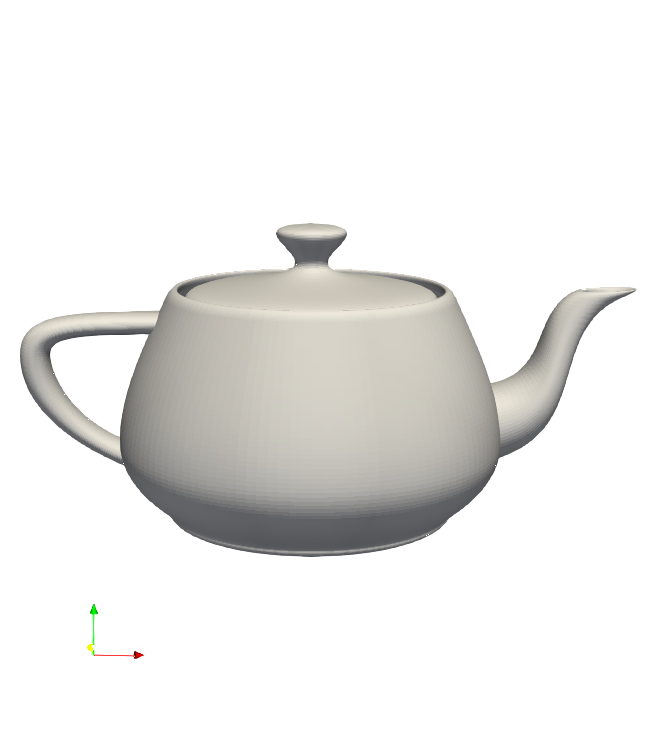
\includegraphics[width=\textwidth]{figures/teapot_geom.png}
        \caption{Multipatch discretization}
        \label{fig:refcase-mesh}
    \end{subfigure}
    \hfill
    \begin{subfigure}[b]{0.32\textwidth}
        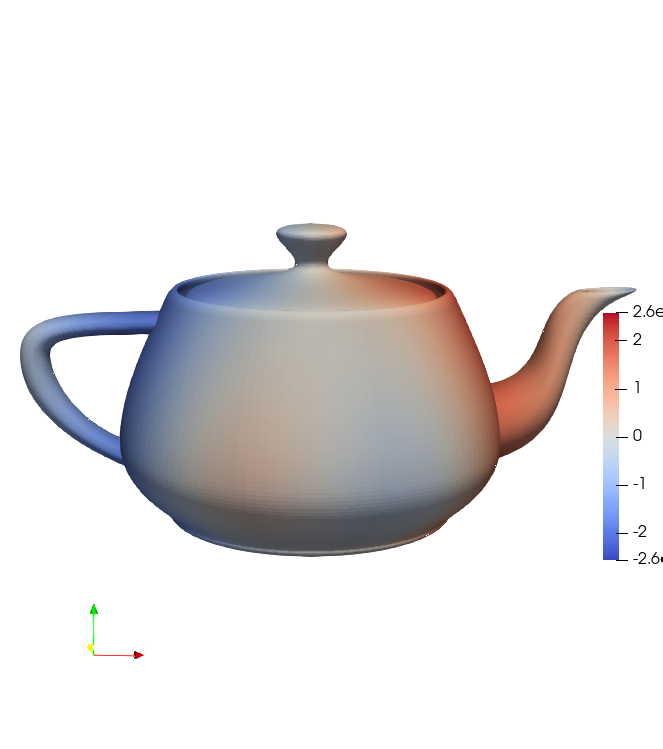
\includegraphics[width=\textwidth]{figures/teapot_rhs.png}
        \caption{Right-hand side}
        \label{fig:refcase-rhs}
    \end{subfigure}
    \hfill
    \begin{subfigure}[b]{0.32\textwidth}
        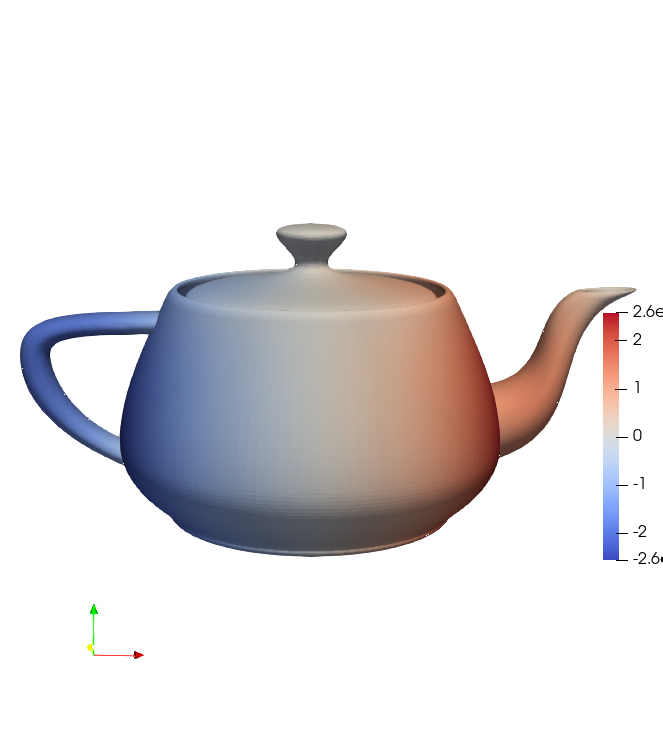
\includegraphics[width=\textwidth]{figures/teapot_sol.png}
        \caption{Computed solution}
        \label{fig:refcase-sol}
    \end{subfigure}
    \caption{Reference case (teapot surface, $32$ patches, $p = 2$, $r = 3$):
    the multipatch discretization, the source term, and the IETI-DP solution.}
    \label{fig:refcase}
\end{figure}

\subsection{Reference case} \label{subsec:bench-reference}

The reference discretization is the teapot surface with $\npatch = 32$ patches
, degree $p = 2$ and refinement $r = 3$ in each patch, giving $N = 2502$
coupled degrees of freedom; the IETI-DP interface problem~\eqref{eq:ieti-schur}
has $\Lambda = 512$ Lagrange multipliers and $\nprim = 22$ primal degrees of
freedom (corner constraints). Table~\ref{tab:reference} reports the results.
Among the iterative solvers, IETI-DP is the fastest: its solve takes
$0.05\,$s, against $0.31\,$s for GMRES and CG preconditioned with multigrid ($6.2\times$
faster) and $0.39\,$s for standalone multigrid ($7.8\times$ faster).

\begin{table}[t]
    \centering
    \caption{Reference case (teapot, $\npatch = 32$, $p = 2$, $r = 3$;
    $N = 2502$). Iterative solvers share the tolerance $10^{-8}$. IETI-DP
    iterations count CG steps on the interface
    problem~\eqref{eq:ieti-schur}, hence are not directly comparable with the
    global-system iteration counts.}
    \label{tab:reference}
    \begin{tabular}{lccc}
        \toprule
        Method &  solve [s] & iters & converged \\
        \midrule
        GMRES (no preconditioner)       &  5.23 & 224  & yes \\
        GMRES + Jacobi                  &  3.66 & 192  & yes \\
        GMRES + symmetric Gauss--Seidel &  0.93 & 80   & yes \\
        GMRES + ILU               &  0.18 & 46 & yes \\
        GMRES + multigrid               &  0.32 & 26   & yes \\
        CG (no preconditioner)       &  0.23 & 346  & yes \\
        CG + Jacobi                  &  0.19 & 207  & yes \\
        CG + symmetric Gauss--Seidel &  0.71 & 90   & yes \\
        CG + ILU               &  2.01 & 1000   & no \\
        CG + multigrid               &  0.31 & 28   & yes \\
        Multigrid (standalone)       &  0.39 & 35   & yes \\
        \textbf{IETI-DP}             &  \textbf{0.05} & 22 & yes \\
        \bottomrule
    \end{tabular}
\end{table}

\subsection{Parameter studies} \label{subsec:bench-sweeps}

We now vary one discretization parameter at a time around the reference case and
record the solve times of IETI-DP and other global solvers
(Figure~\ref{fig:sweeps}). The solve time is the relevant quantity for the
present work: the neural operator~\eqref{eq:neural-schur} replaces the local
Schur-complement action applied once per interface iteration, i.e.\ it acts
within the solve phase, not the assembly.

\begin{figure}[ht!]
    \centering
    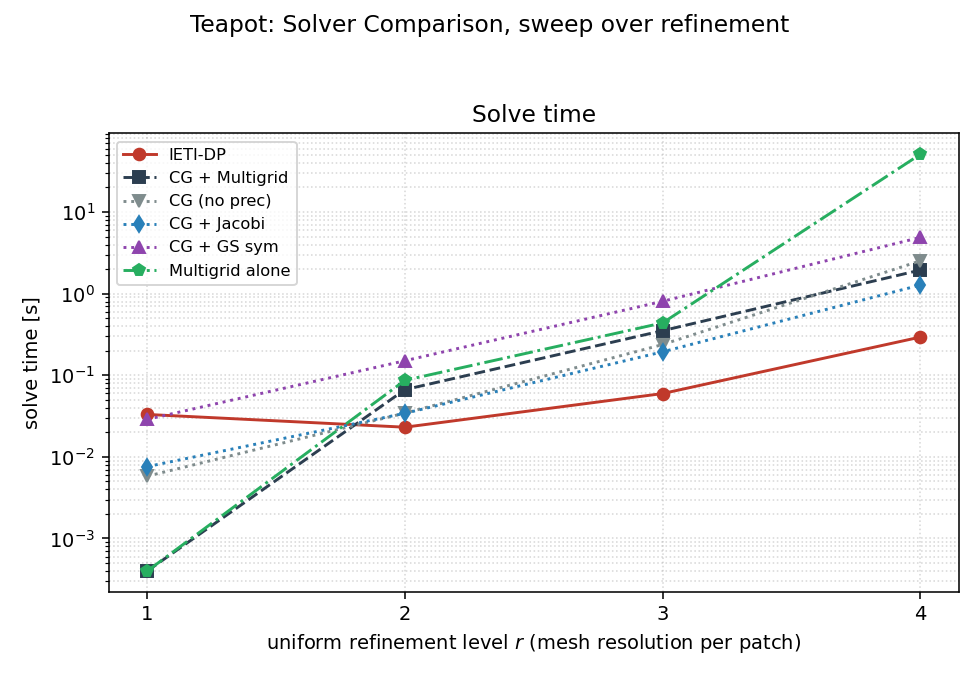
\includegraphics[width=0.8\textwidth]{figures/time_vs_refinement.pdf}
    \caption{Mesh resolution per patch (uniform refinement $r$), at
    $\npatch = 32$, $p = 2$.}
    \label{fig:sweep-refinement}
\end{figure}

\begin{figure}[ht!]
    \centering
    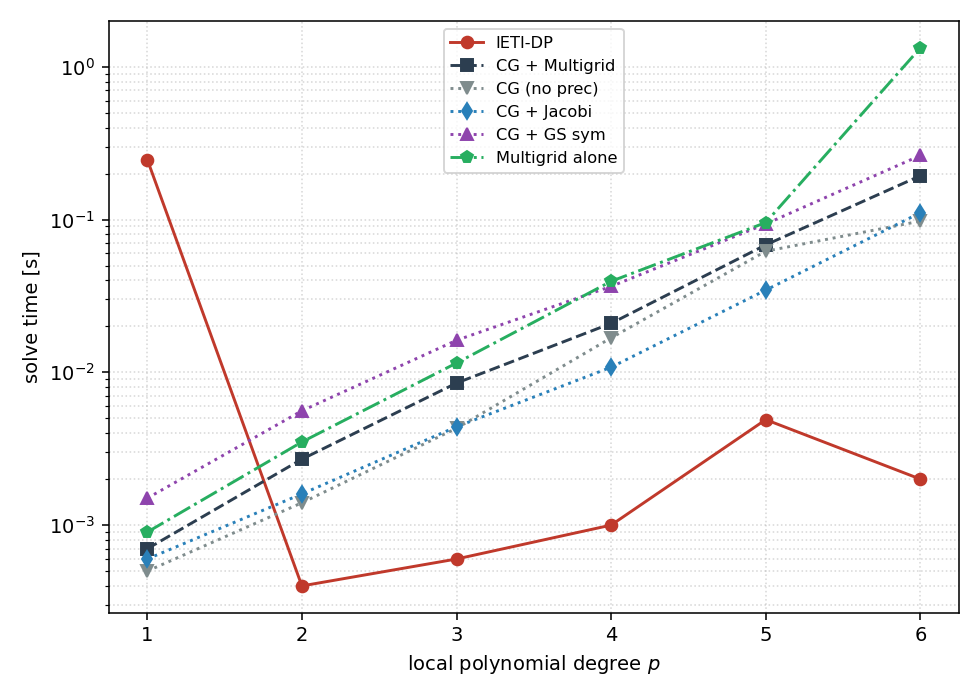
\includegraphics[width=0.8\textwidth]{figures/time_vs_degree.pdf}
    \caption{Local polynomial degree $p$, at $\npatch = 32$, $r = 2$.}
    \label{fig:sweep-degree}
\end{figure}

\begin{figure}[ht!]
    \centering
    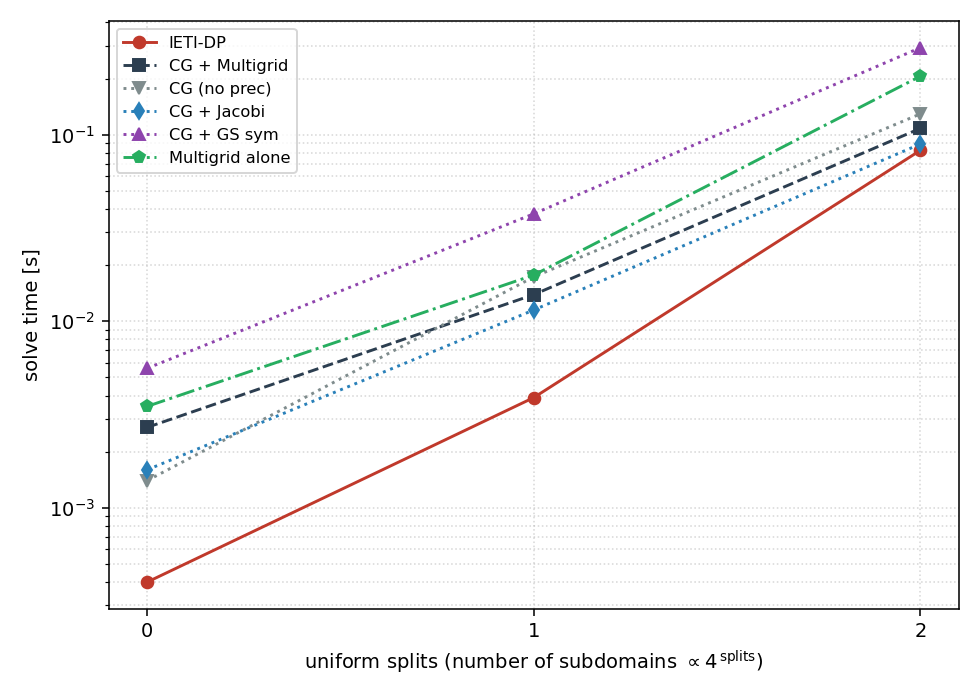
\includegraphics[width=0.8\textwidth]{figures/time_vs_splitpatches.pdf}
    \caption{Number of subdomains (uniform splits), at $p = 2$, $r = 2$.}
    \label{fig:sweep-splitpatches}
\end{figure}

Three trends emerge. \emph{(i)~Mesh resolution}
(Figure~\ref{fig:sweep-refinement}): the IETI-DP solve time grows markedly more
slowly than that of multigrid; multigrid is faster only on the trivially small
$r = 1$ grid ($258$ dofs), and from $r = 2$ onward IETI-DP leads, by $7.4\times$
at $r = 4$ ($0.23\,$s versus $1.68\,$s). \emph{(ii)~Polynomial degree}
(Figure~\ref{fig:sweep-degree}): IETI-DP is faster at every degree and the gap
widens with $p$ (from $2.5\times$ at $p = 1$ to $17\times$ at $p = 4$), the
multigrid smoother degrading as the local spectra spread with degree elevation.
\emph{(iii)~Number of subdomains} (Figure~\ref{fig:sweep-splitpatches}): IETI-DP
is fastest when the subdomains are few and large ($4.8\times$ at $32$ patches,
$3.4\times$ at $128$), but the advantage shrinks as the patches multiply and the
interface problem grows---at $512$ patches the two methods are comparable. This
is the expected behaviour: the cost of~\eqref{eq:ieti-schur} is driven by the
number of Lagrange multipliers and of local solves, both of which scale with the
subdomain count.

The assembly is performed once and is
independent of the solver, whereas the neural preconditioner targets the repeated
solve phase, where IETI-DP already leads in the reference regime (few large
patches) and where the learned operator is designed to reduce the cost further by
replacing each interior solve (Remark~\ref{rmk:schur-cost}) with a single forward
pass.


\subsection{A harder regime: the hummingbird} \label{subsec:bench-hummingbird}

The winner of the IETI-DP/multigrid comparison depends on the subdomain
structure, and the closed hummingbird surface illustrates the opposite regime.
With the default single split it is decomposed into $1248$ small patches, giving
$N = 101090$ coupled degrees of freedom and an interface problem with
$\Lambda = 19968$ Lagrange multipliers; being closed, it carries no Dirichlet
boundary, so the problem is pure Neumann and is regularized as in
Section~\ref{subsec:model}. Here multigrid converges in a single iteration and
solves in $0.18\,$s, whereas IETI-DP needs $45$ interface iterations and
$22.2\,$s: with that many tiny subdomains the interface problem and the
$1248$ per-iteration local solves make IETI-DP far more expensive
(Table~\ref{tab:regimes}). This confirms that IETI-DP is the method of choice in
the few-large-subdomains regime adopted for the reference case, which is the
setting we target with the neural preconditioner.

\begin{table}[t]
    \centering
    \caption{The two regimes. Few large subdomains (teapot) favour IETI-DP; many
    small subdomains (hummingbird) favour multigrid. Solve time [s] with
    iteration count in parentheses.}
    \label{tab:regimes}
    \begin{tabular}{lrrrcc}
        \toprule
        Case & patches & $N$ & $\Lambda$ & CG+multigrid & IETI-DP \\
        \midrule
        Teapot ($p=2$, $r=3$)      & 32   & 2502   & 512   & 0.31 (28) & \textbf{0.045 (22)} \\
        Hummingbird (default)      & 1248 & 101090 & 19968 & \textbf{0.18 (1)} & 22.2 (45) \\
        \bottomrule
    \end{tabular}
\end{table}

%%%%%%%%%%%%%%%%%%%%%%%%%%%%%%%%%%%%%%%%%
%% Bibliography (Harvard notation)
%%%%%%%%%%%%%%%%%%%%%%%%%%%%%%%%%%%%%%%%%
% \clearpage
\begin{thebibliography}{99}
    \bibitem{van2003iterative}
    Van der Vorst, H.A., 2003. Iterative Krylov methods for large linear systems (No. 13). Cambridge University Press.

    \bibitem{kleiss2012ieti}
    Kleiss, S.K., Pechstein, C., Jüttler, B. and Tomar, S., 2012. IETI–isogeometric tearing and interconnecting. Computer methods in applied mechanics and engineering, 247, pp.201-215.

    \bibitem{farhat1991method}
    Farhat, C. and Roux, F.X., 1991. A method of finite element tearing and interconnecting and its parallel solution algorithm. International Journal for Numerical Methods in Engineering, 32(6), pp.1205-1227.

    \bibitem{hofer2018dual}
    Hofer, C. and Langer, U., 2017. Dual-primal isogeometric tearing and interconnecting solvers for multipatch dG-IgA equations. Computer Methods in Applied Mechanics and Engineering, 316, pp.2-21.

    \bibitem{pechstein2013finite}
    Pechstein, C., 2013. Finite and boundary element tearing and interconnecting solvers for multiscale problems. Lecture Notes in Computational Science and Engineering, Vol. 90. Springer.

    \bibitem{wu2026dlhim}
    Wu, Y., van Beek, J.W., Dolean, V. and Heinlein, A., 2026. Are Deep Learning Based Hybrid PDE Solvers Reliable? Why Training Paradigms and Update Strategies Matter. arXiv preprint arXiv:2602.06842.

    \bibitem{Lynch1964}
    Lynch, R.E., Rice, J.R. and Thomas, D.H., 1964. Direct solution of partial difference equations by tensor product methods. Numerische Mathematik, 6(1), pp.185-199.

    \bibitem{de2011geopdes}
    De Falco, C., Reali, A. and Vázquez, R., 2011. GeoPDEs: a research tool for isogeometric analysis of PDEs. Advances in Engineering Software, 42(12), pp.1020-1034.

    \bibitem{de1978practical}
    De Boor, C. and De Boor, C., 1978. A practical guide to splines (Vol. 27, p. 325). New York: springer.

    \bibitem{fanaskov2023spectral}
    Fanaskov, V.S. and Oseledets, I.V., 2023, December. Spectral neural operators. In Doklady Mathematics (Vol. 108, No. Suppl 2, pp. S226-S232). Moscow: Pleiades Publishing.

    \bibitem{montardini2025isogeometric}
    Montardini, M., Takacs, S. and Tani, M., 2025. The Isogeometric Fast Fourier-based Diagonalization method. arXiv preprint arXiv:2512.20269.

    \bibitem{cottrell2009isogeometric}
    Cottrell, J.A., Hughes, T.J. and Bazilevs, Y., 2009. Isogeometric analysis: toward integration of CAD and FEA. John Wiley $\&$ Sons.

    \bibitem{adler2010geometry}
    Adler, R.J., 2010. The geometry of random fields. Society for Industrial and Applied Mathematics.

    \bibitem{saad1993flexible}
    Saad, Y., 1993. A flexible inner-outer preconditioned GMRES algorithm. SIAM Journal on Scientific Computing, 14(2), pp.461-469.

    \bibitem{ghiotto2025hypernos}
    Ghiotto, M., 2025. HyperNOs: automated and parallel library for neural operators research. Bollettino dell'Unione Matematica Italiana, pp.1-35.

    \bibitem{srivastava2014dropout}
    Srivastava, N., Hinton, G., Krizhevsky, A., Sutskever, I. and Salakhutdinov, R., 2014. Dropout: a simple way to prevent neural networks from overfitting. The journal of machine learning research, 15(1), pp.1929-1958.

    \bibitem{math10214014}
    Cui, C., Jiang, K., Liu, Y. and Shu, S., 2022. Fourier neural solver for large sparse linear algebraic systems. Mathematics, 10(21), p.4014.

    \bibitem{vaswani2017attention}
    Vaswani, A., Shazeer, N., Parmar, N., Uszkoreit, J., Jones, L., Gomez, A.N., Kaiser, Ł. and Polosukhin, I., 2017. Attention is all you need. Advances in neural information processing systems, 30.

    \bibitem{he2016identity}
    He, K., Zhang, X., Ren, S. and Sun, J., 2016, September. Identity mappings in deep residual networks. In European conference on computer vision (pp. 630-645). Cham: Springer International Publishing.

    \bibitem{he2016deep}
    He, K., Zhang, X., Ren, S. and Sun, J., 2016. Deep residual learning for image recognition. In Proceedings of the IEEE conference on computer vision and pattern recognition (pp. 770-778).

    \bibitem{kahana2023geometry}
    Kahana, A., Zhang, E., Goswami, S., Karniadakis, G., Ranade, R. and Pathak, J., 2023. On the geometry transferability of the hybrid iterative numerical solver for differential equations. Computational Mechanics, 72(3), pp.471-484.

    \bibitem{kopanivcakova2025deeponet}
    Kopaničáková, A. and Karniadakis, G.E., 2025. Deeponet based preconditioning strategies for solving parametric linear systems of equations. SIAM Journal on Scientific Computing, 47(1), pp.C151-C181.

    \bibitem{brenner2008mathematical}
    Brenner, S.C. and Scott, L.R., 2008. The mathematical theory of finite element methods. New York, NY: Springer New York.

    \bibitem{sampath2010parallel}
    Sampath, R.S. and Biros, G., 2010. A parallel geometric multigrid method for finite elements on octree meshes. SIAM Journal on Scientific Computing, 32(3), pp.1361-1392.

    \bibitem{lee2025hybrid}
    Lee, Y., Florencio, F.L., Pathak, J. and Karniadakis, G.E., 2025. Hybrid Iterative Solvers with Geometry-Aware Neural Preconditioners for Parametric PDEs. arXiv preprint arXiv:2512.14596.

    \bibitem{chen1995universal}
    Chen, T. and Chen, H., 1995. Universal approximation to nonlinear operators by neural networks with arbitrary activation functions and its application to dynamical systems. IEEE transactions on neural networks, 6(4), pp.911-920.

    \bibitem{hughes2005isogeometric}
    Hughes, T.J., Cottrell, J.A. and Bazilevs, Y., 2005. Isogeometric analysis: CAD, finite elements, NURBS, exact geometry and mesh refinement. Computer methods in applied mechanics and engineering, 194(39-41), pp.4135-4195.

    \bibitem{hendrycks2016gaussian}
    Hendrycks, D. and Gimpel, K., 2016. Gaussian error linear units (gelus). arXiv preprint arXiv:1606.08415.

    \bibitem{watanabe2023tree}
    Watanabe, S., 2023. Tree-structured parzen estimator: Understanding its algorithm components and their roles for better empirical performance. arXiv preprint arXiv:2304.11127.

    \bibitem{bergstra2015hyperopt}
    Bergstra, J., Komer, B., Eliasmith, C., Yamins, D. and Cox, D.D., 2015. Hyperopt: a python library for model selection and hyperparameter optimization. Computational Science $\&$ Discovery, 8(1), p.014008.

    \bibitem{li2020massivelyparallelhyperparametertuning}
    Li, L., Jamieson, K., Rostamizadeh, A., Gonina, E., Ben-Tzur, J., Hardt, M., Recht, B. and Talwalkar, A., 2020. A system for massively parallel hyperparameter tuning. Proceedings of machine learning and systems, 2, pp.230-246.

    \bibitem{loshchilov2019decoupledweightdecayregularization}
    Loshchilov, I. and Hutter, F., 2017. Decoupled weight decay regularization. arXiv preprint arXiv:1711.05101.

    \bibitem{sangalli2016isogeometric}
    Sangalli, G. and Tani, M., 2016. Isogeometric preconditioners based on fast solvers for the Sylvester equation. SIAM Journal on Scientific Computing, 38(6), pp.A3644-A3671.

    \bibitem{gahalaut2019condition}
    Gahalaut, K.P., Tomar, S.K. and Douglas, C., 2014. Condition number estimates for matrices arising in NURBS based isogeometric discretizations of elliptic partial differential equations. arXiv preprint arXiv:1406.6808.

    \bibitem{trottenberg2000multigrid}
    Trottenberg, U., Oosterlee, C.W. and Schuller, A., 2001. Multigrid methods. Academic press.

    \bibitem{toselli2004domain}
    Toselli, A. and Widlund, O., 2004. Domain decomposition methods-algorithms and theory (Vol. 34). Springer Science $\&$ Business Media.

    \bibitem{lu2021learning}
    Lu, L., Jin, P., Pang, G., Zhang, Z. and Karniadakis, G.E., 2021. Learning nonlinear operators via DeepONet based on the universal approximation theorem of operators. Nature machine intelligence, 3(3), pp.218-229.

    \bibitem{li2021fourier}
    Li, Z., Kovachki, N., Azizzadenesheli, K., Liu, B., Bhattacharya, K., Stuart, A. and Anandkumar, A., 2020. Fourier neural operator for parametric partial differential equations. arXiv preprint arXiv:2010.08895.

    \bibitem{rahaman2019spectral}
    Rahaman, N., Baratin, A., Arpit, D., Draxler, F., Lin, M., Hamprecht, F., Bengio, Y. and Courville, A., 2019, May. On the spectral bias of neural networks. In International conference on machine learning (pp. 5301-5310). PMLR.

    \bibitem{tielen2020pmultigrid}
    Tielen, R.P.W.M., Möller, M., Göddeke, D. and Vuik, C., 2020. p-multigrid methods and their comparison to h-multigrid methods within Isogeometric Analysis. Computer Methods in Applied Mechanics and Engineering, 372, p.113347.

    \bibitem{moller2026iganet}
    Möller, M., Obermair, G., Singer, I., Gollmann, C., Reali, A. and Elgeti, S., 2026. IGANets: Isogeometric analysis networks and their applications to linear structural analysis problems. Engineering with Computers, 42(3), p.102.

    \bibitem{karniadakis2025nonlinearprec}
    Lee, Y., Liu, S., Darbon, J. and Karniadakis, G.E., 2025. A Neural-Operator Preconditioned Newton Method for Accelerated Nonlinear Solvers. arXiv preprint arXiv:2511.08811.

    \bibitem{karniadakis2025nspod}
    Levrero-Florencio, F., Lee, Y., Pathak, J. and Karniadakis, G.E., 2026. NSPOD: acceleratingthe convergence ofKrylov-based iterative linearsolvers via approximated PODs. arXiv preprint arXiv:2605.07828.

\end{thebibliography}
% \printbibliography

\end{document}
